\documentclass[12pt, titlepage]{article}

\usepackage{fullpage}
\usepackage[round]{natbib}
\usepackage{multirow}
\usepackage{booktabs}
\usepackage{tabularx}
\usepackage{graphicx}
\usepackage{float}
\usepackage{hyperref}
\hypersetup{
    colorlinks,
    citecolor=blue,
    filecolor=black,
    linkcolor=red,
    urlcolor=blue
}

\input{../../Comments}
\input{../../Common}

\newcounter{acnum}
\newcommand{\actheacnum}{AC\theacnum}
\newcommand{\acref}[1]{AC\ref{#1}}

\newcounter{ucnum}
\newcommand{\uctheucnum}{UC\theucnum}
\newcommand{\uref}[1]{UC\ref{#1}}

\newcounter{mnum}
\newcommand{\mthemnum}{M\themnum}
\newcommand{\mref}[1]{M\ref{#1}}

\begin{document}

\title{Module Guide for \progname{}} 
\author{\authname}
\date{\today}

\maketitle

\pagenumbering{roman}

\section{Revision History}

\begin{tabularx}{\textwidth}{p{3cm}p{2cm}X}
\toprule {\bf Date} & {\bf Version} & {\bf Notes}\\
\midrule
2025-01-xx & 1.0 & Initial version\\
\bottomrule
\end{tabularx}

\newpage

\section{Reference Material}

This section records information for easy reference.

\subsection{Abbreviations and Acronyms}

\renewcommand{\arraystretch}{1.2}
\begin{tabular}{l l} 
  \toprule		
  \textbf{symbol} & \textbf{description}\\
  \midrule 
  AC & Anticipated Change\\
  API & Application Programming Interface\\
  DAG & Directed Acyclic Graph \\
  DSP & Digital Signal Processing\\
  I/O & Input/Output\\
  M & Module \\
  MG & Module Guide \\
  MIDI & Musical Instrument Digital Interface\\
  MIS & Module Interface Specification\\
  NFR & Non-Functional Requirement\\
  OS & Operating System \\
  PDF & Portable Document Format\\
  R & Requirement\\
  SRS & Software Requirements Specification\\
  UC & Unlikely Change\\
  UI & User Interface\\
  XML & eXtensible Markup Language\\
  \progname & An audio to sheet music generator \\
  \bottomrule
\end{tabular}\\

\newpage

\tableofcontents

\listoftables

\listoffigures

\newpage

\pagenumbering{arabic}

\section{Introduction}
Decomposing a system into modules is a commonly accepted approach to developing
software.  A module is a work assignment for a programmer or programming
team~\citep{ParnasEtAl1984}.  We advocate a decomposition
based on the principle of information hiding~\citep{Parnas1972a}.  This
principle supports design for change, because the ``secrets'' that each module
hides represent likely future changes.  Design for change is valuable in SC,
where modifications are frequent, especially during initial development as the
solution space is explored.  

Our design follows the rules layed out by \citet{ParnasEtAl1984}, as follows:
\begin{itemize}
\item System details that are likely to change independently should be the
  secrets of separate modules.
\item Each data structure is implemented in only one module.
\item Any other program that requires information stored in a module's data
  structures must obtain it by calling access programs belonging to that module.
\end{itemize}

After completing the first stage of the design, the Software Requirements
Specification (SRS), the Module Guide (MG) is developed~\citep{ParnasEtAl1984}. The MG
specifies the modular structure of the system and is intended to allow both
designers and maintainers to easily identify the parts of the software.  The
potential readers of this document are as follows:

\begin{itemize}
\item New project members: This document can be a guide for a new project member
  to easily understand the overall structure and quickly find the
  relevant modules they are searching for.
\item Maintainers: The hierarchical structure of the module guide improves the
  maintainers' understanding when they need to make changes to the system. It is
  important for a maintainer to update the relevant sections of the document
  after changes have been made.
\item Designers: Once the module guide has been written, it can be used to
  check for consistency, feasibility, and flexibility. Designers can verify the
  system in various ways, such as consistency among modules, feasibility of the
  decomposition, and flexibility of the design.
\end{itemize}

The rest of the document is organized as follows. Section
\ref{SecChange} lists the anticipated and unlikely changes of the software
requirements. Section \ref{SecMH} summarizes the module decomposition that
was constructed according to the likely changes. Section \ref{SecConnection}
specifies the connections between the software requirements and the
modules. Section \ref{SecMD} gives a detailed description of the
modules. Section \ref{SecTM} includes two traceability matrices. One checks
the completeness of the design against the requirements provided in the SRS. The
other shows the relation between anticipated changes and the modules. Section
\ref{SecUse} describes the use relation between modules. Section \ref{SecUI} illustrates the design 
of the user interface through drawings, sketches, and design tool prototyping 
(e.g. Figma, Marvel, etc.). Section \ref{SecCP} describes the design of communication protocols 
used by the system, in the case of ScoreGen, this section is not relevant. Finally, section 
\ref{SecTL} outlines the schedule of tasks related to the development of ScoreGen as well as the 
development team members responsible for these tasks.

\section{Anticipated and Unlikely Changes} \label{SecChange}

This section lists possible changes to the system. According to the likeliness
of the change, the possible changes are classified into two
categories. Anticipated changes are listed in Section \ref{SecAchange}, and
unlikely changes are listed in Section \ref{SecUchange}.

\subsection{Anticipated Changes} \label{SecAchange}

Anticipated changes are the source of the information that is to be hidden
inside the modules. Ideally, changing one of the anticipated changes will only
require changing the one module that hides the associated decision. The approach
adapted here adheres to the development principle called design for change.

\begin{description}
  \item[\refstepcounter{acnum} \actheacnum \label{acHardware}:] The specific hardware on which the software is running.
  \item[\refstepcounter{acnum} \actheacnum \label{acExtractionMapping}:] Musical element extraction and mapping techniques.
  \item[\refstepcounter{acnum} \actheacnum \label{acMonophonic}:] Monophonic audio processing algorithm(s).
  \item[\refstepcounter{acnum} \actheacnum \label{acComplex}:] Complex audio processing algorithm(s).
  \item[\refstepcounter{acnum} \actheacnum \label{acPerformance}:] Performance and latency benchmarks and targets.
\end{description}
  
\subsection{Unlikely Changes} \label{SecUchange}

The module design aims to be as general as possible. If some design decisions
should need to be changed later, then many parts of the design
will potentially need to be modified. Hence, it is not intended that these
decisions will be changed.

\begin{description}
  \item[\refstepcounter{ucnum} \uctheucnum \label{ucInputFormat}:] File format of input data.
  \item[\refstepcounter{ucnum} \uctheucnum \label{ucOutputFormat}:] File format of output audio data.
  \item[\refstepcounter{ucnum} \uctheucnum \label{ucEditing}:] Post-generation editing and progress saving.
  \item[\refstepcounter{ucnum} \uctheucnum \label{ucNotation}:] Choice of sheet music notation.
  \item[\refstepcounter{ucnum} \uctheucnum \label{ucUI}:] User interface features, requirements, usability, styling, etc.
  \item[\refstepcounter{ucnum} \uctheucnum \label{nfrStability}:] Non-functional requirements are unlikely to change.
\end{description}

\section{Module Hierarchy} \label{SecMH}

This section provides an overview of the module design. Modules are summarized
in a hierarchy decomposed by secrets in Table \ref{TblMH}. The modules listed
below, which are leaves in the hierarchy tree, are the modules that will
be implemented.

\begin{description}
\item [\refstepcounter{mnum} \mthemnum \label{mHH}:] Hardware-Hiding Module
\item [\refstepcounter{mnum} \mthemnum \label{mUI}:] User Interface Module
\item [\refstepcounter{mnum} \mthemnum \label{mSG}:] Score Generation Module
\item [\refstepcounter{mnum} \mthemnum \label{mRSM}:] Raw Signal Processing Module
\item [\refstepcounter{mnum} \mthemnum \label{mAFE}:] Audio Feature Extraction Module
\item [\refstepcounter{mnum} \mthemnum \label{mFFC}:] File Format Conversion Module
\item [\refstepcounter{mnum} \mthemnum \label{mARP}:] Audio Recording/Playback Module
\end{description}

\begin{table}[h!]
  \centering
  \begin{tabular}{p{0.3\textwidth} p{0.6\textwidth}}
  \toprule
  \textbf{Level 1} & \textbf{Level 2}\\
  \midrule
  
  {Hardware-Hiding Module} & -\\
  \midrule
  
  \multirow{3}{0.3\textwidth}{Behaviour-Hiding Module} 
  & User Interface Module \\
  & Score Generation Module \\
  & File Format Conversion Module \\
  \midrule
  
  \multirow{3}{0.3\textwidth}{Software Decision Module} 
  & Raw Signal Processing Module \\
  & Audio Feature Extraction Module \\
  & Audio Recording and Playback Module \\
  \bottomrule
  
  \end{tabular}
  \caption{Module Hierarchy}
  \label{TblMH}
\end{table}
  

\section{Connection Between Requirements and Design} \label{SecConnection}

The design of the system is intended to satisfy the requirements developed in
the SRS. In this stage, the system is decomposed into modules. The connection
between requirements and modules is listed in Table~\ref{TblRT}.

\section{Module Decomposition} \label{SecMD}

Modules are decomposed according to the principle of ``information hiding''
proposed by \citep{ParnasEtAl1984} . The \emph{Secrets} field in a module
decomposition is a brief statement of the design decision hidden by the
module. The \emph{Services} field specifies \emph{what} the module will do
without documenting \emph{how} to do it. For each module, a suggestion for the
implementing software is given under the \emph{Implemented By} title. If the
entry is \emph{OS}, this means that the module is provided by the operating
system or by standard programming language libraries. \emph{\progname{}} means the
module will be implemented by the \progname{} software.
Only the leaf modules in the hierarchy will be implemented. If a dash
(\emph{--}) is shown, this means that the module is not a leaf and will not have
to be implemented.

\subsection{Hardware Hiding Module (\mref{mHH})}

\begin{description}
\item[Secrets:]The data structure and algorithm used to implement the virtual
  hardware.
\item[Services:]Serves as a virtual hardware used by the rest of the
  system. This module provides the interface between the hardware and the
  software. So, the system can use it to display outputs or to accept inputs.
\item[Implemented By:] OS
\end{description}

\subsection{Behaviour-Hiding Modules}

\begin{description}
\item[Secrets:] The contents of the required behaviours.
\item[Services:] Includes programs that provide externally visible behaviour of
  the system as specified in the software requirements specification (SRS)
  documents. This module serves as a communication layer between the
  hardware-hiding module and the software decision module. The programs in this
  module will need to change if there are changes in the SRS.
\item[Implemented By:] --
\end{description}

\subsubsection{User Interface Module (\mref{mUI})}

\begin{description}
\item[Secrets:] Style and layout standards, user input management, and event- and display-handling.
\item[Services:] Provides the user with an intuitive, graphical interface for interacting with the system.
  Maps user input to appropriate system functions. Dynamically updates the display to reflect user interactions.
\item[Implemented By:] ScoreGen.
\item[Type of Module:] Unsure
\end{description}

\subsubsection{Score Generation Module (\mref{mSG})}

\begin{description}
\item[Secrets:] Musical notation standards and conventions used by the system.
\item[Services:] Ends the audio to sheet music transcription pipeline by providing the user with viewable, human-readable sheet music.
  Maps pre-processed audio data to elements used by viewable or exportable file formats such as MusicXML, PDF, etc.
  Renders the viewable sheet music for the UI to display to the user.
\item[Implemented By:] ScoreGen.
\item[Type of Module:] Library, contains reusable routines.
\end{description}

\subsubsection{File Format Conversion Module (\mref{mFFC})}

\begin{description}
\item[Secrets:] Details of reading and writing to files in order to perform conversions from one file format to another.
\item[Services:] Converts files to other supported formats (e.g., PDF to MIDI).
\item[Implemented By:] OS, external libraries.
\item[Type of Module:] Library, contains reusable routines for file format conversions.
\end{description}

\subsection{Software Decision Modules}

\begin{description}
\item[Secrets:] The design decision based on mathematical theorems, physical
  facts, or programming considerations. The secrets of this module are
  \emph{not} described in the SRS.
\item[Services:] Includes data structure and algorithms used in the system that
  do not provide direct interaction with the user. 
\item[Implemented By:] --
\end{description}

\subsubsection{Raw Signal Processing Module (\mref{mRSM})}

\begin{description}
\item[Secrets:] The underlying mathematical and physical principles that govern sound waves and their transformation into digital representations.
  Techniques used to transform time domain audio signals into the frequency domain.
\item[Services:] Digital signal processing.
  Takes in raw audio data and transforms them into frequency domain representations.
  Provides the system with data prepared for subsequent audio feature extraction.
\item[Implemented By:] External libraries.
\item[Type of Module:] Library, contains reusable methods for digital signal processing.
\end{description}

\subsubsection{Audio Feature Extraction Module (\mref{mAFE})}

\begin{description}
\item[Secrets:] The techniques and algorithms chosen to derive pitch, key signature, rhythm, and timing from frequency domain data.
\item[Services:] Detection and classification of musical elements such as pitches, key signature, rhythm, and timing.
  Identifies pitches based on dominant frequencies.
  Classifies musical characteristics including key signature, rhythm, and timing.
  Provides the system with data prepared for subsequent score generation.
\item[Implemented By:] External libraries.
\item[Type of Module:] Library, contains reusable methods for extracting musical elements from pre-processed data.
\end{description}

\subsubsection{Audio Recording and Playback Module (\mref{mARP})}

\begin{description}
\item[Secrets:] Audio input and output management and related device-specific configurations.
\item[Services:] Allows the user to capture audio with a device of their choosing and to listen to their recordings.
  Sets and configures input and output streams for the device ScoreGen is running on.
  User-directed recording (i.e. start, stop, playback).
\item[Implemented By:] OS, external libraries.
\item[Type of Module:] Library, contains reusable routines for accessing and configuring audio I/O.
\end{description}

\section{Traceability Matrix} \label{SecTM}

This section shows two traceability matrices: between the modules and the
requirements and between the modules and the anticipated changes.

% the table should use mref, the requirements should be named, use something
% like fref
\begin{table}[H]
\centering
\begin{tabular}{p{0.2\textwidth} p{0.6\textwidth}}
\toprule
\textbf{Req.} & \textbf{Modules}\\
\midrule
FR-AI1 & \mref{mHH}, \mref{mARP}\\
FR-AI2 & \mref{mARP}\\
FR-AI3 & \mref{mUI}, \mref{mRSM}\\
FR-AI4 & \mref{mUI}\\
FR-SP1 & \mref{mRSM}\\
FR-SP2 & \mref{mAFE}\\
FR-SP3 & \mref{mAFE}\\
FR-SP4 & \mref{mRSM}\\
FR-SP5 & \mref{mRSM}\\
FR-SP6 & \mref{mRSM}\\
FR-SMG1 & \mref{mSG}, \mref{mAFE}\\
FR-SMG2 & \mref{mSG}, \mref{mAFE}\\
FR-SMG3 & \mref{mUI}, \mref{mSG}\\
FR-UI1 & \mref{mUI}, \mref{mARP}\\
FR-UI2 & \mref{mUI}\\
FR-UI3 & \mref{mUI}\\
FR-UI4 & \mref{mUI}\\
FR-SL1 & \mref{mUI}, \mref{mFFC}\\
FR-SL2 & \mref{mUI}, \mref{mFFC}\\
\bottomrule
\end{tabular}
\caption{Trace Between Requirements and Modules}
\label{TblRT}
\end{table}

\begin{table}[H]
\centering
\begin{tabular}{p{0.2\textwidth} p{0.6\textwidth}}
\toprule
\textbf{AC} & \textbf{Modules}\\
\midrule
\acref{acHardware} & \mref{mHH}\\
\acref{acExtractionMapping} & \mref{mAFE}\\
\acref{acMonophonic} & \mref{mRSM}\\
\acref{acComplex} & \mref{mRSM}\\
\acref{acPerformance} & \mref{mRSM}\\
\bottomrule
\end{tabular}
\caption{Trace Between Anticipated Changes and Modules}
\label{TblACT}
\end{table}

\section{Use Hierarchy Between Modules} \label{SecUse}

In this section, the uses hierarchy between modules is
provided. \citet{Parnas1978} said of two programs A and B that A {\em uses} B if
correct execution of B may be necessary for A to complete the task described in
its specification. That is, A {\em uses} B if there exist situations in which
the correct functioning of A depends upon the availability of a correct
implementation of B.  Figure \ref{FigUH} illustrates the use relation between
the modules. It can be seen that the graph is a directed acyclic graph
(DAG). Each level of the hierarchy offers a testable and usable subset of the
system, and modules in the higher level of the hierarchy are essentially simpler
because they use modules from the lower levels.

\begin{figure}[H]
\centering
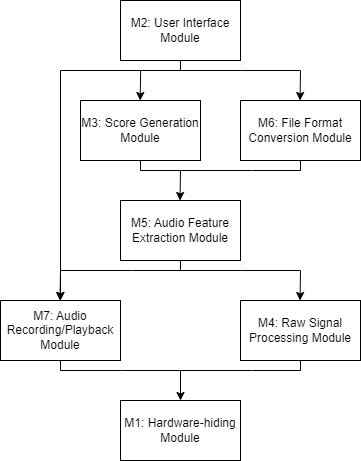
\includegraphics[width=0.5\textwidth]{./images/ModuleGuideUseHierarchy.jpg}
\caption{Use hierarchy among modules}
\label{FigUH}
\end{figure}

%\section*{References}

\section{User Interfaces} \label{SecUI}
\begin{itemize}
  \item Rough ideas for design in Figma is available at \href{https://www.figma.com/design/CWFjGlXuaUj9XEe1k2O9HN/ScoreGen?node-id=8-16&t=teQzB6fJFKylFmIW-1}{this link}.
  \item Logo design is available at \href{https://www.canva.com/design/DAGb84uW3qQ/pLjQfILAEV3cagekQF9ojQ/edit?utm_content=DAGb84uW3qQ&utm_campaign=designshare&utm_medium=link2&utm_source=sharebutton}{this link}.
\end{itemize}

\section{Design of Communication Protocols} \label{SecCP}

N/A.

\section{Timeline} \label{SecTL}
The following table breaks down the tasks that must be completed in order to 
accurately implement all modules of the software.

\begin{table}[H]
  \centering
  \begin{tabular}{p{0.3\textwidth} p{0.3\textwidth} p{0.25\textwidth}}
  \toprule
  \textbf{Task} & \textbf{Developer} & \textbf{Completion Date}\\
  \midrule
  \mref{mUI} Implementation & Jackson & Jan 20/25\\
  \mref{mUI} Unit Testing & Jackson & Jan 27/25\\
  \mref{mSG} Implementation & Ian & Jan 20/25\\
  \mref{mSG} Unit Testing & Ian & Jan 27/25\\
  \mref{mRSM} Implementation & Emily, Ian & Nov 15/24\\
  \mref{mRSM} Unit Testing & Emily, Ian & Jan 27/25\\
  \mref{mAFE} Implementation & Emily, Ian, Mark, Jackson & Jan 20/25\\
  \mref{mAFE} Unit Testing & Emily, Ian, Mark, Jackson & Jan 27/25\\
  \mref{mFFC} Implementation & Mark & Jan 20/25\\
  \mref{mFFC} Unit Testing & Mark & Jan 27/25\\
  \mref{mARP} Implementation & Emily & Jan 11/25\\
  \mref{mARP} Unit Testing & Emily & Jan 27/25\\
  Integration Testing & Emily, Ian, Mark, Jackson & Feb 3/25\\
  \bottomrule
  \end{tabular}
  \caption{Task Completion Timeline}
  \label{TblSched}
  \end{table}

\bibliographystyle{plainnat}
\bibliography{../../../refs/References}

\newpage{}

\end{document}